\newcommand{\ttH}{\ensuremath{t\bar{t}H}}
\newcommand{\pt}{\ensuremath{p_{T}}}
\newcommand{\ptH}{\ensuremath{\pt^{H}}}

\newcommand{\tH}{\ensuremath{tH}}
\newcommand{\tHW}{\ensuremath{tHW}}
\newcommand{\tHQ}{\ensuremath{tHq}}
\newcommand{\VH}{\ensuremath{VH}}
\newcommand{\ggH}{\ensuremath{gg\rightarrow H}}
\newcommand{\mgg}{\ensuremath{m_{\gamma\gamma}}}
\newcommand{\ptgg}{\ensuremath{\pt^{\gamma\gamma}}}

\newcommand{\hgg}{\ensuremath{H\rightarrow\gamma\gamma}}


\begin{center}
\textit{Wardle,~Langford}
\end{center}


As detailed in the previous section, an alternative approach to probing the Higgs boson self-coupling is to measure deviations of the inclusive and differential Higgs boson production rates. Contributions to single Higgs boson production from the Higgs boson self-coupling are sizeable for production in association with a pair of top quarks ($\ttH$) or a single top-quark ($\tH$). The contributions are  greatest in these production modes due to the large mass of the top quark. Differential cross section measurements, in particular as a function of the Higgs boson 
transverse momentum $\pt^{H}$, allow one to disentangle the effects of modified Higgs boson self-coupling values from 
other effects such as the presence of anomalous top--Higgs couplings.  

This section describes the strategy for measuring the differential $\pt$ cross section for 
Higgs boson production in association with at least one top quark, and decaying to photons ($\ttH+\tH$, $\hgg$), 
at the High-Luminosity LHC (HL-LHC) with the CMS Phase-2 detector. The $\hgg$ decay mode provides a final state in which the decay of the Higgs boson can be fully reconstructed, and a direct measurement of the $\pt$ differential cross-section can be made. 

The expected precision of the analysis is determined based on simulated proton-proton ($pp$) events, at a centre of mass energy of 14 TeV.
Simulated signal and background events are generated using a combination of {\sc POWHEG}
v2.0~\cite{Alioli:2010xd,Nason:2009ai}, {\sc MADGRAPH5\_AMC@NLO} v2.2.2~\cite{Alwall:2014hca}, {\sc SHERPA} v2.2.5~\cite{Gleisberg:2008ta}, and interfaced with {\sc PYTHIA} v8.205~\cite{Sjostrand:2007gs}. The signal and background events are processed with {\sc DELPHES}~\cite{deFavereau2014}, using the CMS Phase-2 card, to simulate the response of the upgraded CMS detector to showered particles. 

The differential cross-section measurements are used to extract a 
constraint on the Higgs boson self-coupling ($\lambda_{3}$), by parameterising deviations from SM predictions as described in the previous section. The kinematic dependance of these deviations are determined by reweighting signal events, on an event by event basis,  using the tool described in Ref.~\cite{EWreweightingtool}, which calculates $\lambda_3$-dependent corrections to the tree level cross-sections as a function of the kinematic properties of the event.  Full details of the analysis can be found in Ref.~\cite{REF TO CMS PAS}


\subsection{Analysis strategy}

An event selection is applied to the simulated background and signal events following a similar strategy to the CMS run-2 $\hgg$ strategy. The events are required to contain two photons, with $|\eta^\gamma|$~$<$~2.4 excluding the region 1.44~$<$~$|\eta^\gamma|$~$<$~1.57, with an invariant mass satisfying 100~$<$~$\mgg$~$<$~180~GeV, where the leading-$\pt$ (sub-leading-$\pt$) photon satisfies $\pt^{\gamma}/\mgg$~$>$~1/3 (1/4). The two photons are also required to be separated by $\Delta R_{\gamma\gamma}$~$>$~0.4. The photons must also be isolated, which is achieved by requiring that the sum of charged transverse momentum in a cone of radius $\Delta R_{\gamma}$~=~0.4, centred on the photon direction, is less than 0.3$\, \pt^\gamma$. For events where more than one photon pair passes the selection, then the pair with $\mgg$ closest to the Higgs boson mass is chosen.

In order to isolate the production of the Higgs boson in association with top quarks, the selection requires all events to have at least one $b-$tagged jet. Such events are separated into two orthogonal categories based on the decay products of the top quark, a hadronic category and a leptonic category. In the hadronic category, events must contain at least 3 jets, clustered using the anti-$k_{T}$ algorithm with a cone size of 0.4, separated by $\Delta R$~$>$~0.4 with respect to both photon candidates. The jets are required to have $\pt>25$ GeV and $|\eta|$~$<$~4. In the leptonic category, only 2 jets are required, however, in addition, at least one isolated muon or electron in the event. The muons or electrons must satisy $\pt$~$>$~20~GeV and $|\eta|$~$<$~2.4, excluding the region 1.44~$<$~$|\eta^\gamma|$~$<$~1.57 for electrons. The muons must satisfy an isolation requirement that the sum of all reconstructed particles $\pt$, inside a cone of radius $\Delta R=0.4$, excluding the muon itself, is less than 0.25 times the transverse momentum of the muon. In addition, for electrons, the invariant mass of pairs formed from the electron and either selected photon, $m_{e\gamma}$, is required to be greater than 95 GeV to reduce contamination from $Z\rightarrow e^{+}e^{-}$ decays. Events which as selected in the leptonic category are excluded from the hadronic selection to maintain orthogonality of the two categories.  
For the signal extraction boosted decision tree (BDT) classifiers are trained independently in each channel, which distinguish between signal-like and background-like events, using input variables related to the kinematics of the events, such as the lepton and jet momenta and pseudo-rapidities, and the scalar sum of transverse momentum of all final state objects in the event. Events are required to have output BDT values greater than some threshold which are tuned to provide the best sensitivity to $\kappa_{\lambda}$. The hadronic category is further split into two different regions of BDT output, for events with diphoton transverse momentum ($\ptgg$) less than 350 GeV, to reduce the contamination of $\ggH$ events. 

Finally, the events are further divided into six bins of $\ptgg$, given in Tab.~\ref{tab:ttHdiff_CMS_ptbins}, making a total of 17 categories. 

\begin{table}[h]

 \centering
 \begin{tabular}{c|c|c|c|c|c|c}
 %{P{1cm}P{1cm}P{1cm}P{1cm}P{1cm}P{1cm}P{1cm}}
  %\hline
    \multicolumn{7}{c}{$\ptH$ or $\ptgg$ bin boundaries (GeV)}  \\ \hline
    0 & 45 & 80 & 120 & 200 & 350 & $\infty$ \\\hline
\end{tabular}
\caption{bin boundaries which define the $\ptH$ regions for which the differential cross sections are measured. These also correspond to the bins in which the hadronic and leptonic event categories are sub-divided.}
\label{tab:ttHdiff_CMS_ptbins}
\end{table}

Experimental systematic uncertainties are included in the signal model, which can cause migration both between the different categories and in and out of the fiducial region. The dominant experimental uncertainties include uncertainties in the reconstruction and 
identification efficiencies for photons and b jets as well as uncertainties on the energy scale and resolution of reconstructed jets. 
Furthermore, theoretical uncertainties are included on the rates of $\ggH$ and $\VH$ contamination, which modify both the overall normalisation and the relative contamination between the different categories for these processes. The background estimation will be determined directly from the mass sidebands in the data and therefore the uncertainties on the background will be entirely statistical in nature. However, the impact of increasing the rate of fake photons in the background component has been studied and was found to reduce the sensitivity to $\kappa_\lambda$ by roughly 10\% when in the worst case scenario.  

\subsection{Differential cross-section results}

In order to account for resolution effects, the signal events are separated based on the $\ptH$ at generator level.   Signal and background models are constructed using the simulated events in each category. The signal model accounts for the relative populations of events from the different production processes as well as from different $\ptH$ bins, and the diphoton mass resolution expected from events in each category. The background model is constructed from a fit of smoothly falling functions to the weighted sum of simulated background samples, accounting for the different fake photon rates for each source of background. The differential cross-section is determined from and a simultaneous maximum likelihood fit to an Asimov data set corresponding to $3ab^{-1}$, and assuming SM Higgs boson  production in each category.  Systematic uncertainties are accounted for through the introduction of constrained nuisance parameters in the log-likelihood, which are profiled. 

The results of this fit are given in figure~\ref{fig:ttHdiff_CMS_ptH_xs}. The results shown are unfolded back to a fiducial region which is common to both the hadronic and leptonic selections, and shown using only the hadronic or leptonic categories, and their combination. The theoretical uncertainties displayed on the predicted $\ttH+\tH$ cross section are calculated by modifying the renormalisation and factorisaton scales up and down by a factor of 2.

\begin{figure}[htb!]
        \centering
        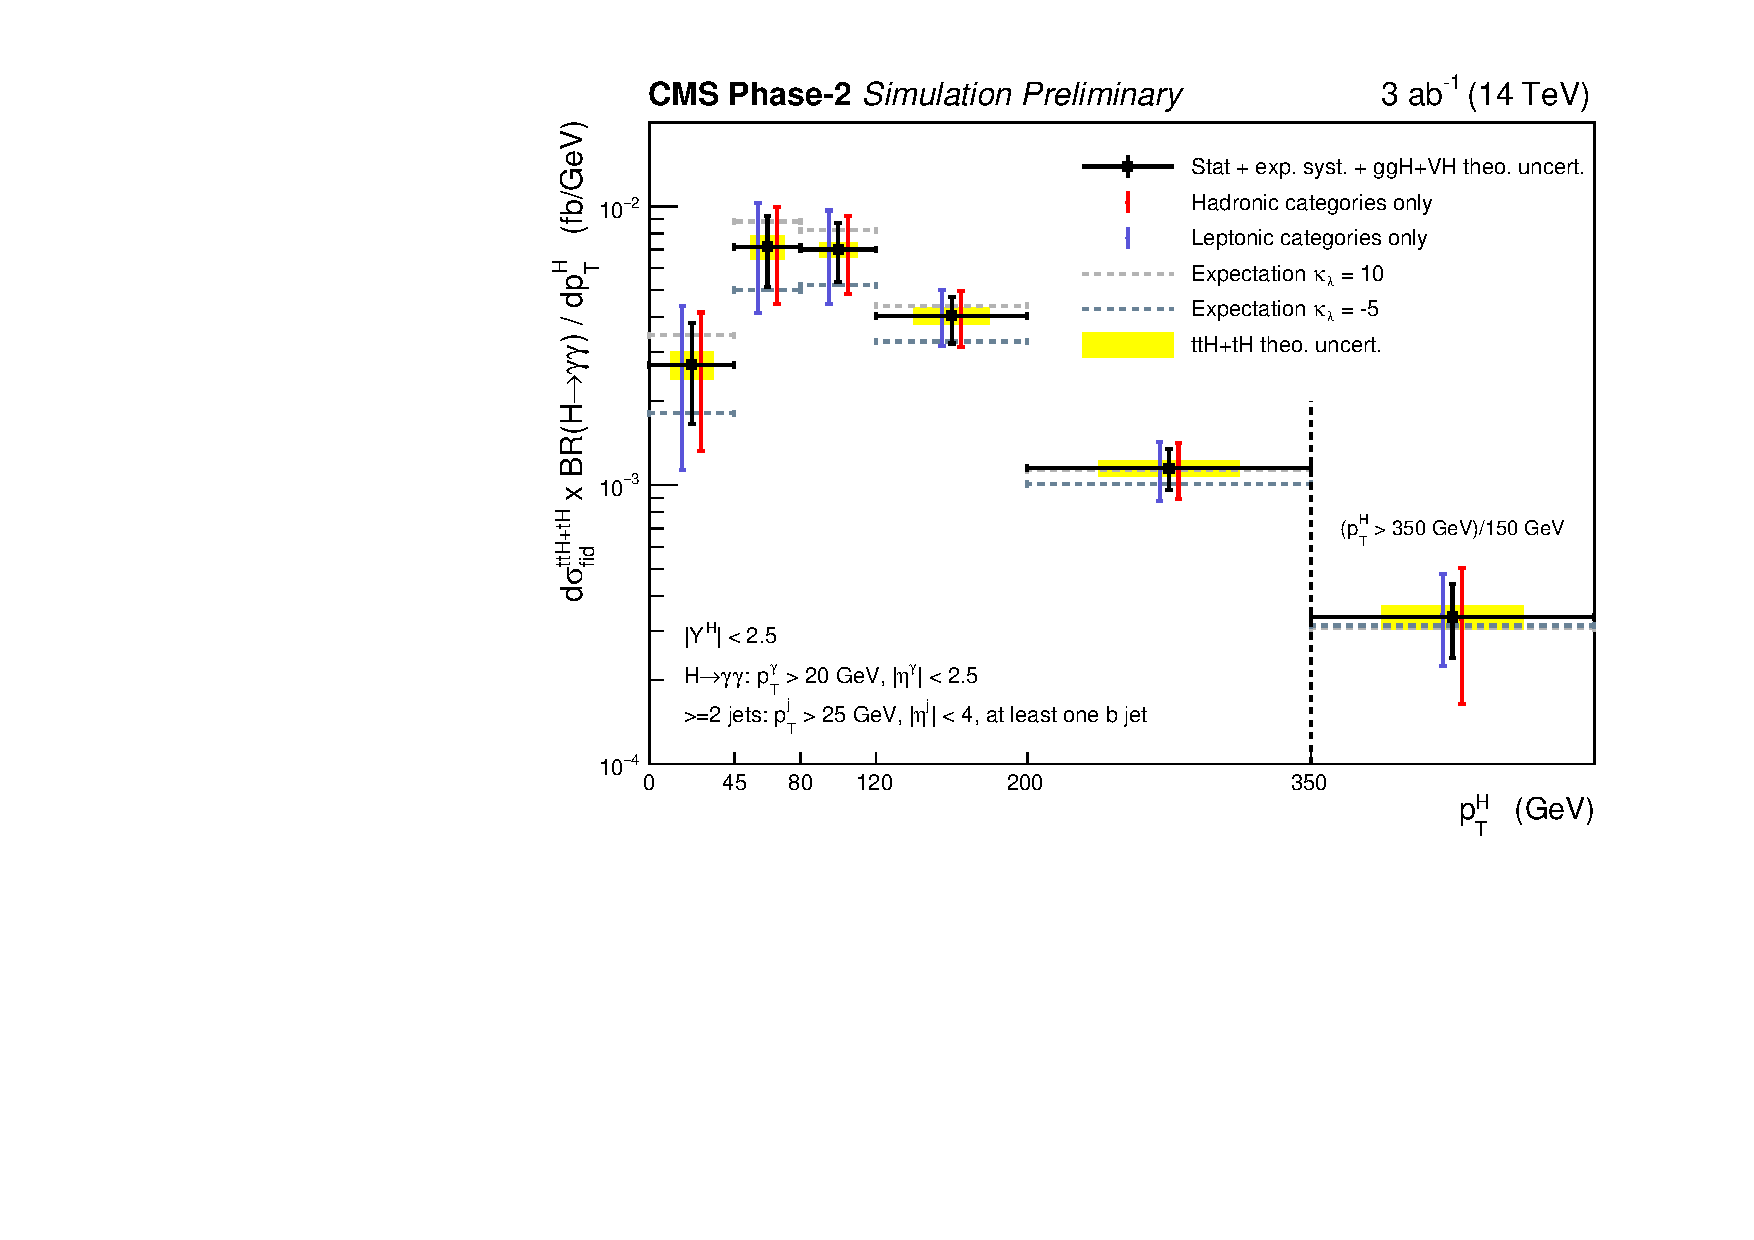
\includegraphics[width=0.6\textwidth]{\main/section3/plots/dXS_dpTH.pdf}
        \caption{The expected $\ptH$ differential $\ttH$~+~$\tH$ cross sections times branching ratio, along with their uncertainties. The error bars on the black points include the statistical uncertainty, the experimental systematic uncertainties and the theoretical uncertainties related to the $\ggH$ and $\VH$ contamination, which is subtracted in the fit.  The cross section for $\ptH>350$ GeV is scaled by the width of the previous bin. The expected $\ttH$~+~$\tH$ cross sections for anomalous values of the Higgs boson self-coupling ($\kappa_\lambda$~=~10 and $\kappa_\lambda$~=~-5) are shown by the horizontal dashed lines.}
        \label{fig:ttHdiff_CMS_ptH_xs}
\end{figure}

\subsection{Constraints on the Higgs boson self coupling}

Modifications to the differential cross section for $\ttH$~+~$\tH$ production can be parameterised as a function of $\kappa_\lambda$ using the reweighting tool provided in Ref.~\cite{EWreweightingtool}. The value of $C_{1}$ depends on the Higgs boson production mode and the kinematic properties of the event. Table~\ref{tab:ttHdiff_CMS_c1_values} shows the values of $C_1$ calculated in the fiducial region for $\ttH$ and $\tH$ production, in each bin of $\ptH$.

\begin{table}[t!]
\begin{center}
\begin{tabular}{|c |c| c| c| c| c| c|}
\hline
   $p_T(H)$~[GeV] & $[0, 45]$  & $[45, 80]$ & $[80, 120]$ & $[120, 200]$ &  $[200, 350]$ &  $>350$ \\ 
\hline
\hline
ttH & $5.31$ & $4.73$ & $3.92$ & $2.79$ & $1.42$ & $0.42$ \\
\hline
tH & $1.32$ &$1.19$ & $1.00$ & $0.75$ & $0.40$ & $0.06$ \\
\hline 
VH & $1.66$ & $1.23$ & $0.77$ & $0.35$ & $0.02$ & $-0.09$ \\
\hline
\end{tabular}
 \caption{Process dependant $C_{1}$ values for each bin of $\ptH$.}
\label{tab:ttHdiff_CMS_c1_values}
\end{center}
\end{table}


In addition, the contribution from $\VH$ production is included by similarly calculating the $C_{1}$ values for $\VH,~\hgg$ events. For the contribution of $\ggH$ and to account for modifications of the $\hgg$ decay width, the parameterisations which have been calculated for inclusive events provided in Ref.~\cite{Degrassi:2016wml} are used directly.

Figure~\ref{fig:ttHdiff_CMS_klambda_scan} shows a scan of the profile log-likelihood, as a function of $\kappa_{\lambda}$, is shown in . In the scan, all other Higgs boson couplings are assumed to attain their SM values. For the purposes of constraining $\kappa_{\lambda}$, the theoretical uncertainties in the differential $\ttH$~+~$\tH$ cross section, as described in the previous sub-section, are included in the signal model. The results when only including the hadronic or leptonic categories are shown in addition to the result obtained from their combination. 

\begin{figure}[htb!]
        \centering
        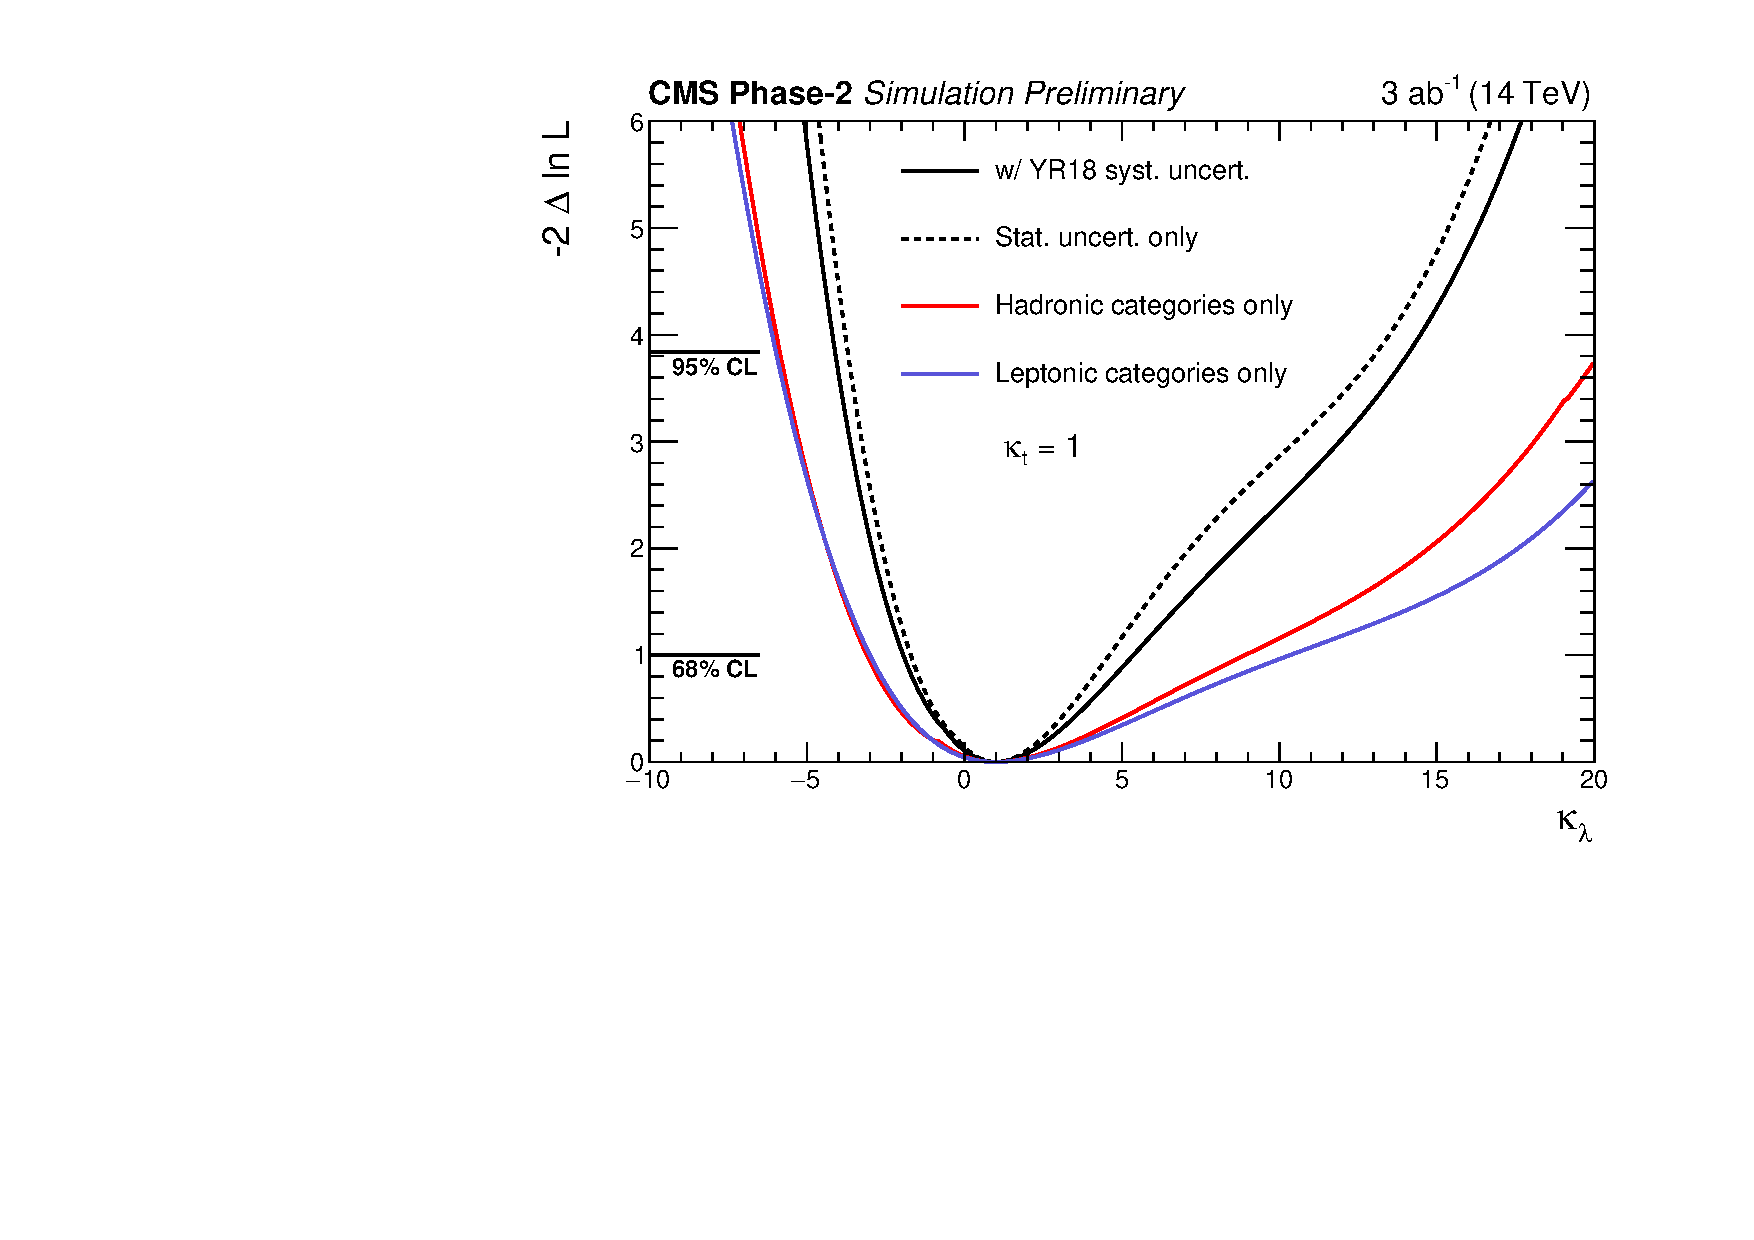
\includegraphics[width=0.6\textwidth]{\main/section3/plots/klambda_scan.pdf}
        %\vspace{2mm}
        \caption{Profile log-likelihood scan as a function of $\kappa_\lambda$. The individual contributions of the statistical and systematic uncertainties are separated by performing a likelihood scan with all systematics removed. Additionally, the contributions from the hadronic and leptonic channels have been separated, shown in red and purple, respectively.}
        \label{fig:ttHdiff_CMS_klambda_scan}
\end{figure}


The profiled log-likelihood in the region around 
$5<\kappa_\lambda<15$ results from the behaviour of the parameterisations which modify the predicted cross sections. For the $\ttH$ production mode, the derivative of the predicted cross section with respect to $\kappa_\lambda$ changes sign in this region, such that the predicted cross section is relatively stable for different values of $\kappa_\lambda$. This degeneracy is however somewhat resolved by the  other production modes for which the change in sign occurs at different values of $\kappa_\lambda$. With $3ab^{-1}$ of data collected by CMS at the HL-LHC, this result shows that a constraint of $-4.1 < \kappa_\lambda < 14.1$ at the 95\% confidence level (CL) is acheivable from the differential cross-section measurement of a single Higgs boson decay channel produced in association with tops, using data from only one of the two general purpose detectors at the HL-LHC.  


The $\ttH$~+~$\tH$ differential cross section measurements are also sensitive to other potential BSM effects, such as those which give rise to anomalous top--Higgs couplings. A two-dimensional profile log-likelihood scan is shown in  Fig.~\ref{fig:ttHdiff_CMS_klambda_2Dscan} as a function of $\kappa_\lambda$ and $\mu_{H}$. The parameter $\mu_{H}$ is a multiplicative scaling factor which is common to all Higgs boson production modes and all $\ptH$ bins. Even with this additional parameter, constraints on $\kappa_\lambda$ are still achievable, owing to the information retained in the shape of the $\ptH$ distribution. The constraint on $\kappa_\lambda$ is $-7.1 < \kappa_\lambda < 14.1$ at the 95\% CL, when the log-likelihood is also profiled with respect to $\mu_{H}$. 

\begin{figure}[htb!]
        \centering
        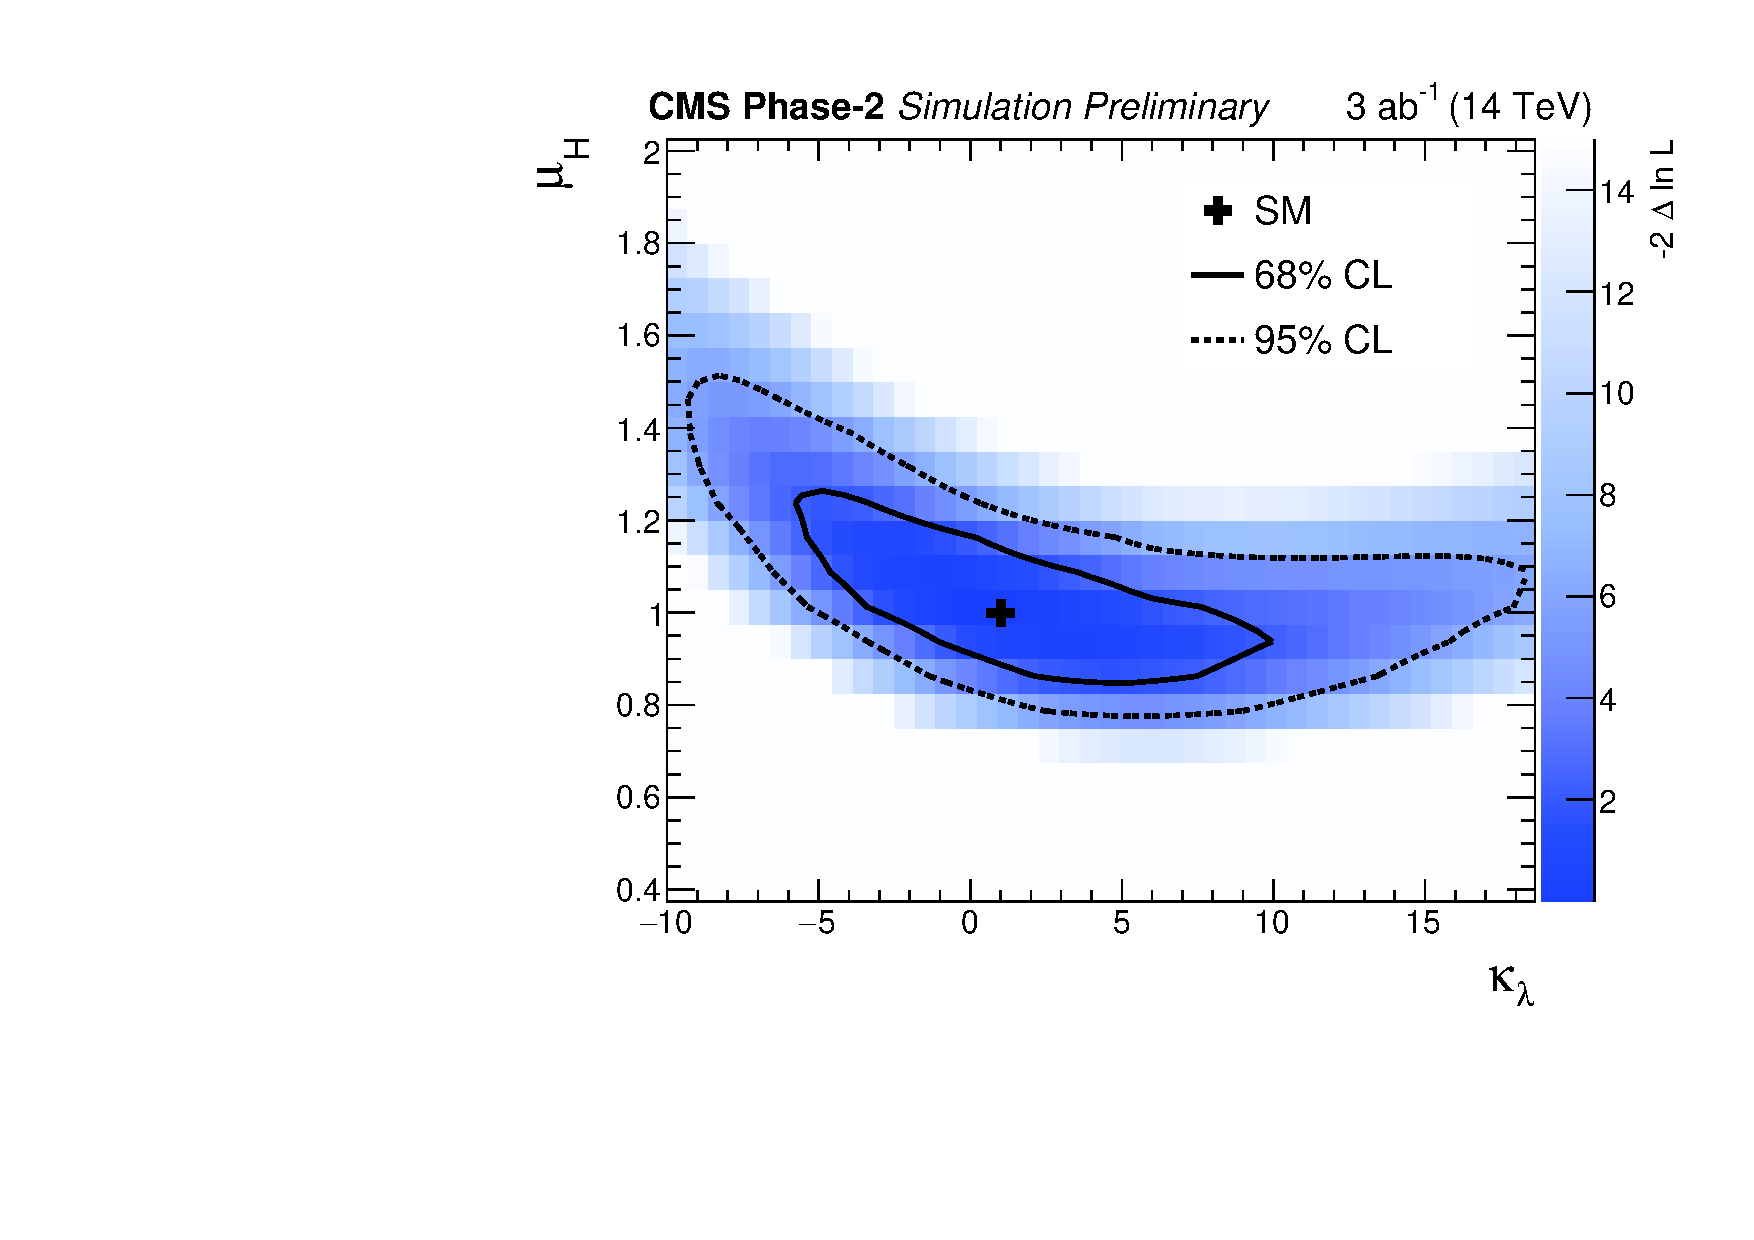
\includegraphics[width=0.6\textwidth]{\main/section3/plots/2D_kappa_mu_scan.pdf}
        %\vspace{2mm}
        \caption{Results of the two-dimensional likelihood scan in $\kappa_\lambda$-vs-$\mu_{H}$, where $\mu_{H}$ allows all Higgs boson production modes to scale relative to the SM prediction. The 68\% and 95\% confidence level contours are shown by the solid and dashed lines respectively. The SM expectation is shown by the black cross.}
        \label{fig:ttHdiff_CMS_klambda_2Dscan}
\end{figure}


